\begin{answer}
\begin{figure}[H]
    \centering
    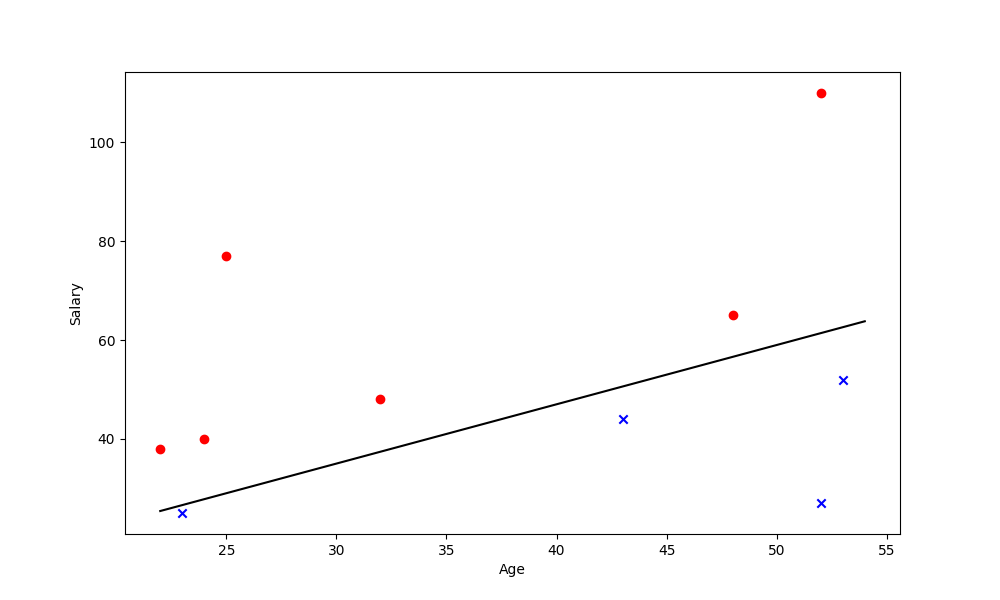
\includegraphics[width=10.5cm]{decision_trees_general/check.png}
\end{figure}
As, we observe from the plot above, the data is separable by the line 
$x_{\text{income}} = -1 + 1.2x_{\text{age}}$
Therefore, by setting $\alpha=-1.2$, $\beta=1$, we get 100\% accuracy if we split by the sign of $\alpha x_{\text{age}} +\beta x_{\text{income}} -1$ at the root node. The error reduction of the split is, thus $\frac{4}{10}$
\end{answer}